\newpage
\section{Methodology}\label{methodology}

\subsection{CA-Based Fire Model}

Our wildfire model is constructed using a two-dimensional $m$-by-$n$ matrix, corresponding to $m\times n$ individual square cells. Each cell in the matrix has an assigned integer value representing its state, with definitions shown in Table \ref{table:cellstates}:

\begin{table}[h!]
    \centering
    \begin{tabular}{|c|c|}
    \hline
     \textbf{Cell Value} & \textbf{Cell State} \\ \hline
     0 & Cell is flammable, corresponds to vegetation\\ \hline
     1 & Cell is not flammable, corresponds to bare terrain and water\\ \hline
     2 & Cell is on fire, will keep burning for a fixed amount of time\\ \hline
     3 & Cell is burnt, corresponds to a fire that has stopped burning\\ \hline
    \end{tabular}
    \caption{Cell values and their meanings used in fire simulation}
    \label{table:cellstates}
\end{table}

\noindent We define a matrix of cell values to simplify the simulated system into an array of four possible states: vegetation, non-flammable terrain, fire and burnt fuel. This matrix evolves in discrete time steps through a set of fixed rules as specified in Section \ref{ruleset}, representing the time evolution of the fire system.

\subsection{Rules for Evolution}\label{ruleset}

The simulation is performed by calculating the cell array for $N$ time steps, where the future value of each cell is determined by the current state of a neighbourhood, comprised of the given cell and a fixed number of cells in its proximity. Our method uses the 9-cell Moore neighbourhood, which balances computation speed with physical accuracy \cite{Wolfram_2002}. The rules of evolution for each discrete state from 0 to 4 are presented in Table \ref{table:futurestate}:

\begin{table}[h!]
    \centering
    \begin{tabular}{|c|c|}
    \hline
     \textbf{Current State ($t=t_0$)} & \textbf{Future State ($t=t_0+1$)}\\ \hline
     0 & 0 OR 2\\ \hline
     1 & 1\\ \hline
     2 & 2 OR 3\\ \hline
     3 & 3\\ \hline
    \end{tabular}
    \caption{Rules of fire evolution in cell array for discrete states 0 to 3}
    \label{table:futurestate}
\end{table}

\noindent Our model assumes that a fuel cell has a finite probability of catching fire, depending on the exact configuration of its neighbourhood. Fuel cells ignite with a probability $P(0\xrightarrow{}2)=p$, and remain intact with a probability $P(0\xrightarrow{}0) = 1- p$. If a cell is on fire, it will remain on fire until a specific amount of time steps has passed, determined by the fire duration $\Delta t$. The state of a non-flammable cell is static over time, remaining non-flammable for the entire simulation. Likewise, a cell that is burnt remains burnt for the duration of the simulation. To model the physical environment of fire, we calculate the probability of ignition $p$ using specified environmental variables as described in Section \ref{factors}.
\subsection{Environmental Factors}\label{factors}
The spread of fire is influenced by a sizeable number of physical factors, most determined by the exact geographical conditions at the time of fire. To create a simulation with non-trivial predictive power without requiring an unfeasible amount of computational power, our model is restricted to four major variables: elevation, wind speed, wind direction and spotting\footnote{Spotting is the phenomenon by which sparks or embers from an active fire are carried by wind to start new fires}. We define the ignition probability $p$ of a fuel cell $C$ as a function of individual probability factors $p_e$, $p_w$ and $p_s$, for elevation, wind and spotting respectively. The resulting probability of ignition $p$ is defined by:

\begin{equation}\label{netp}
    p = \begin{cases} \sqrt{p_e p_w}, & \mbox{if } C \mbox{ has neighbours on fire} \\ p_s, & \mbox{otherwise}
     \end{cases}
\end{equation}

\noindent where the square root appears for normalisation. To simplify the calculations we assume that the probability of ignition due to a cell's immediate neighbours is much larger than ignition due to spotting, $\sqrt{p_e p_w}\gg p_s$, allowing us to treat the two cases as independent. This simplifies the model and improves computation speed at the marginal loss of accuracy.\newline
\indent To calculate the elevation probability $p_e$, we use a relation derived by D. Weise \textit{et al.} in 1998 \cite{Weise_1998}. Observations show that fire has a greater rate of spread when travelling uphill compared to that of fire travelling downhill. This can be modelled using an exponential function of the elevation angle $\theta$. The elevation ignition probability $p_e$ is defined by:

\begin{equation}\label{p_elevation}
    p_e = C_1\times\sum_{i=1}^8\exp(\alpha\theta_i)
\end{equation}

\noindent where $\alpha$ is a strength parameter determining how strongly the gradient angle $\theta$ affects the ignition probability for each cell in the Moore neighbourhood for $i = 1,...,8$, and $C_1$ is a normalisation constant. For the value $\alpha=0$, the elevation change has no effect on ignition probability, and for $\alpha > 0$ the elevation has an increasing effect. The gradient angle $\theta$ is calculated using the relation:

\begin{equation}\label{theta_elevation}
        \theta = \begin{cases} \arctan{\left(\frac{h_1 - h_2}{d}\right)}, & \mbox{for adjacent cells} \\ \arctan{\left(\frac{h_1 - h_2}{\sqrt{2}d}\right)}, & \mbox{for diagonal cells}
     \end{cases}
\end{equation}

\noindent where $h_1$ is the height of the centre cell, $h_2$ is the height of the neighbour cell, and $d$ is the width of a cell in the array. Due to the square grid, a factor of $\sqrt{2}$ is included for diagonal cells. \newline \indent The effect of wind is implemented using a similar relationship, based on an exponential dependence between fire transition probability and the angle normal to the wind direction. We use a modification of the method developed by A. Aleksandridis \textit{et al.} in their 2008 paper \cite{Aleksandridis_2008}, and calculate the transition probability of fire $p_w$ to a specific fuel cell using:
\begin{equation} \label{p_wind}
    p_w = C_2 \times \sum_{i=1}^{8}\exp(\beta \times \mathbf{w} \cdot \mathbf{r}_i)
\end{equation}

\noindent where we take the sum for all neighbour cells with indices $i = 1,...,8$, $\beta$ is a wind strength parameter, $\mathbf{w}$ is the wind velocity vector, $\mathbf{r}_i$ is the direction from the middle cell to the neighbour cell $i$, and $C_2$ is a normalisation constant. The parameter $\beta$ determines the degree to which wind affects the fire transition probability, where $\beta=0$ means the wind has no effect on fire transition and $\beta>0$ has an increasing effect.\newline
\indent The third environmental factor we implement is spotting, and it affects all fuel cells in the cell array. We develop a novel method of simulating the diffusion-type behaviour of flying embers through a Gaussian convolution process, allowing us to describe the spotting phenomenon via a probabilistic approach. An example of a possible ember distribution is presented in Figure \ref{fig:emberFig}, where the heat map displays the concentration of embers in each cell before and after Gaussian convolution.

\begin{figure}[h]
\centering
    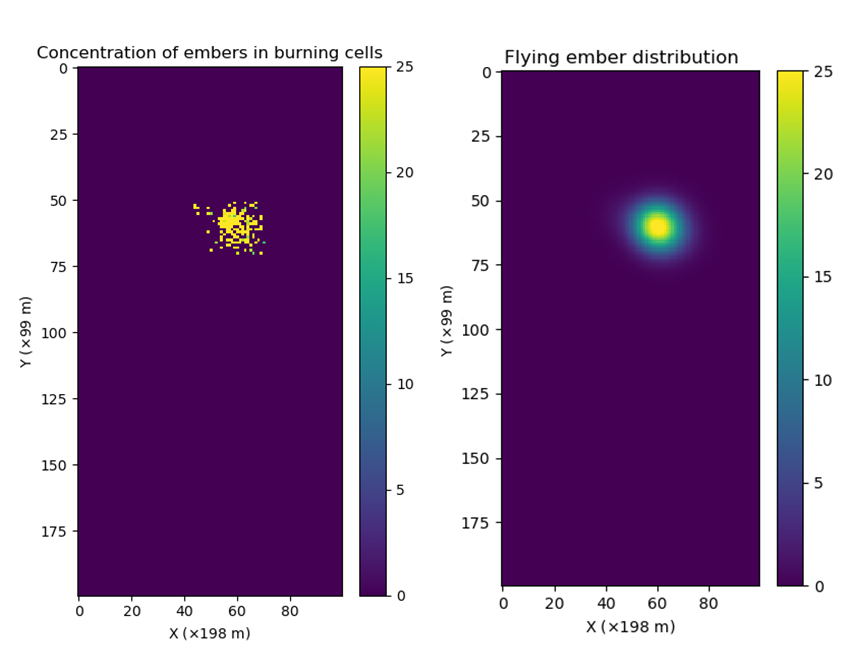
\includegraphics[width=0.95\textwidth]{Figures/embers_comp.png}
    \caption{Left: initial distribution of embers emitted by each burning cell. Right: final distribution of embers after applying Gaussian convolution. Heat map range: from 0 embers per cell (purple) to 25 embers per cell (yellow).}
    \label{fig:emberFig}
\end{figure}

\noindent  The final distribution represents the probability that an ember has landed on a given cell, thus allowing us to calculate the ignition probability $p_s$ of a fuel cell due to spotting. To obtain this distribution, we assume that each burning cell emits on average a number $E$ embers carried by wind. This process is described by a  Poisson distribution with a mean value $E$, where we pick a random value from the distribution to represent the embers emitted by each cell at each time step. The embers are carried by wind, and their spread across the landscape is modelled using a Gaussian convolution kernel with a radius $R$ given by:
\begin{equation}\label{convolution}
    R = t_{f}\times \abs{\mathbf{w}}
\end{equation}
where $t_f$ is the time that an ember remains on fire in the air, and $\mathbf{w}$ is the wind velocity vector. To ensure that the kernels travel along the direction of the wind, this process is performed along the wind vector for a length $R$. To obtain the ember ignition probability, we assume that each fuel cell has an associated normal distribution representing the number of embers required to ignite a fire in the cell. The mean and standard deviation of this distribution are defined as $M$ and $\sigma$ respectively. We obtain a relationship for the ignition probability of any cell due to the spotting effect, denoted by $p_s$:

\begin{equation}\label{p_spotting}
    p_s(x) = \frac{1}{2}\left[1 + \erf\left(\frac{x-M}{\sigma \sqrt{2}}\right)\right]\\
\end{equation}

\noindent where $\erf$ is the Gauss error function, and $x$ is the number of embers that have landed on the cell after the convolution process. To simplify the computational requirements of this calculation, we defined a discrete range of $x$-values for which the ignition probability is calculated. We define $p_s(x)$ such that $p_s(M+3\sigma) \approx 1$, and $p_s(M-3\sigma) \approx 0$, and the values of $x$ within these limits are rounded to the nearest decimal point. This trade-off sacrifices marginal accuracy for a substantial computational speed gain. \newline
\indent In addition to incorporating these environmental effects, the model can also use a simple alternative rule set. To do this, the cellular automaton in our code can be defined such that the ignition probability $p$ of a fuel cell $C$ at index $i$ in the array is given by:
\begin{equation}\label{p_ignition}
    p = \frac{1}{8} \times \sum_{i=1}^8 C(i) \delta_{C(i),2}
\end{equation}
where the index $i = 1,...,8$ belongs to the Moore neighbourhood of the cell $C$, a cell on fire is represented by $C(i)=2$ and $\delta$ is the Kronecker delta function. This expression gives us the simple relation $p=F/8$, where $F$ is the number of neighbouring cells on fire. To revert to this calculation for the ignition probabilities, the elevation and wind strength parameters are normalised. This means that for an arbitrary wind and elevation input, if $\alpha,\beta=0$ then the ignition probability $p$ is calculated according to Equation \ref{p_ignition}.

\subsection{Simulation Environment}

We use Python v3.7.4 as our main simulation environment, with Numpy v1.17 and Scipy v1.4.1 as additional packages. The source data for vegetation, wind and elevation is processed using MATLAB R2019b with the Mapping Toolbox\texttrademark{} and the Image Processing Toolbox\texttrademark{}. An overview of the Python code is given as a class diagram in Appendix \ref{code}, and the source data is acquired through Geoscience Australia's Web Portal \cite{Geodata}.